\documentclass[a4paper,titlepage,11pt,twosides,floatssmall]{mwrep}
\usepackage[left=2.5cm,right=2.5cm,top=2.5cm,bottom=2.5cm]{geometry}
\usepackage[OT1]{fontenc}
\usepackage{polski}
\usepackage{amsmath}
\usepackage{amsfonts}
\usepackage{amssymb}
\usepackage{graphicx}
\usepackage{url}
\usepackage{tikz}
\usetikzlibrary{arrows,calc,decorations.markings,math,arrows.meta}
\usepackage{rotating}
\usepackage[percent]{overpic}
\usepackage[utf8]{inputenc}
\usepackage{xcolor}
\usepackage{pgfplots}
\usetikzlibrary{pgfplots.groupplots}
\usepackage{listings}
\usepackage{matlab-prettifier}
\definecolor{szary}{rgb}{0.95,0.95,0.95}
\usepackage{siunitx}
\usepackage{placeins}
\sisetup{detect-weight,exponent-product=\cdot,output-decimal-marker={,},per-mode=symbol,binary-units=true,range-phrase={-},range-units=single}
\SendSettingsToPgf
%konfiguracje pakietu listings
\lstset{
	backgroundcolor=\color{szary},
	frame=single,
	breaklines=true,
}
\lstdefinestyle{customlatex}{
	basicstyle=\footnotesize\ttfamily,
	%basicstyle=\small\ttfamily,
}
\lstdefinestyle{customc}{
	breaklines=true,
	endframe=tb,
	language=C,
	xleftmargin=0pt,
	showstringspaces=false,
	basicstyle=\small\ttfamily,
	keywordstyle=\bfseries\color{green!40!black},
	commentstyle=\itshape\color{purple!40!black},
	identifierstyle=\color{blue},
	stringstyle=\color{orange},
}
\lstdefinestyle{custommatlab}{
	captionpos=t,
	breaklines=true,
	frame=tb,
	xleftmargin=0pt,
	language=matlab,
	showstringspaces=false,
	%basicstyle=\footnotesize\ttfamily,
	basicstyle=\scriptsize\ttfamily,
	keywordstyle=\bfseries\color{green!40!black},
	commentstyle=\itshape\color{purple!40!black},
	identifierstyle=\color{blue},
	stringstyle=\color{orange},
}

%wymiar tekstu (bez żywej paginy)
\textwidth 160mm \textheight 247mm

%ustawienia pakietu pgfplots
\pgfplotsset{
tick label style={font=\scriptsize},
label style={font=\small},
legend style={font=\small},
title style={font=\small}
}

\def\figurename{Rys.}
\def\tablename{Tab.}

%konfiguracja liczby pływających elementów
\setcounter{topnumber}{0}%2
\setcounter{bottomnumber}{3}%1
\setcounter{totalnumber}{5}%3
\renewcommand{\textfraction}{0.01}%0.2
\renewcommand{\topfraction}{0.95}%0.7
\renewcommand{\bottomfraction}{0.95}%0.3
\renewcommand{\floatpagefraction}{0.35}%0.5

\begin{document}
\frenchspacing
\pagestyle{uheadings}

%strona tytułowa
\title{\bf Sprawozdanie z ćwiczenia laboratoryjnego nr 5 \vskip 0.1cm}
\author{Mateusz Koroś, Ksawery Pasikowski, Mateusz Morusiewicz}
\date{2017}

\makeatletter
\renewcommand{\maketitle}{\begin{titlepage}
\begin{center}{\LARGE {\bf
Wydział Elektroniki i Technik Informacyjnych}}\\
\vspace{0.4cm}
{\LARGE {\bf Politechnika Warszawska}}\\
\vspace{0.3cm}
\end{center}
\vspace{5cm}
\begin{center}
{\bf \LARGE Projektowanie układów sterowania\\ (projekt grupowy) \vskip 0.1cm}
\end{center}
\vspace{1cm}
\begin{center}
{\bf \LARGE \@title}
\end{center}
\vspace{2cm}
\begin{center}
{\bf \Large \@author \par}
\end{center}
\vspace*{\stretch{6}}
\begin{center}
\bf{\large{Warszawa, \@date\vskip 0.1cm}}
\end{center}
\end{titlepage}
}
\makeatother

\maketitle

\tableofcontents


\chapter{Zad. 1}
Możliwość sterowania i pomiaru w komunikacji ze stanowiskiem została sprawdzona poprzez funkcję readMeasurements, sendControls oraz sendNonLinearControls. Sygnały sterujące, które były obsługiwane to moce na grzałkach $G1$ i $G2$ (wysłana za pomocą funkcji sendNonLinearControls) oraz moce wiatraków $ W1 $ i $ W2 $(wysłana za pomocą sendControls), natomiast mierzone były temperatury $ T1 $ i $ T3 $ w otoczeniach grzałek odpowiednio $ G1 $ i $ G2 $. W punkcie pracy, tzn. dla $ (W1, W2, G1, G2) = (50, 50, 29, 34) $ pomiary temperatur wyniosły $(T1, T3) = (36, 38)$.
\begingroup
\renewcommand{\cleardoublepage}{}
\renewcommand{\clearpage}{}


\chapter{Zad. 2}
Na sterowniku został zaimplementowany mechanizm zabezpieczający przed uszkodzeniem stanowiska. Został on napisany w języku ST i był stosowany ze wszystkimi regulatorami.


\endgroup

\chapter{Zad. 3}

Na sterowniku został zaimplementowany reguator PID, w języku ST. Kod jest dostępny w pliku programu gxworks3. Zostały dobrane następujące nastawy: $K = 6$, $Ti = 65$, $Td = 1.25$. Wykres pokazuje działanie regulatora dla skoku wartości zadanych $T1_{zad} = 40, T3_{zad} = 42$. Regulator PID stosunkowo szybko dochodzi do wartości zadanej ($11 minut$) oraz ma akceptowalne przeregulowanie ($3°C$).

\begin{figure}[]
	\centering
	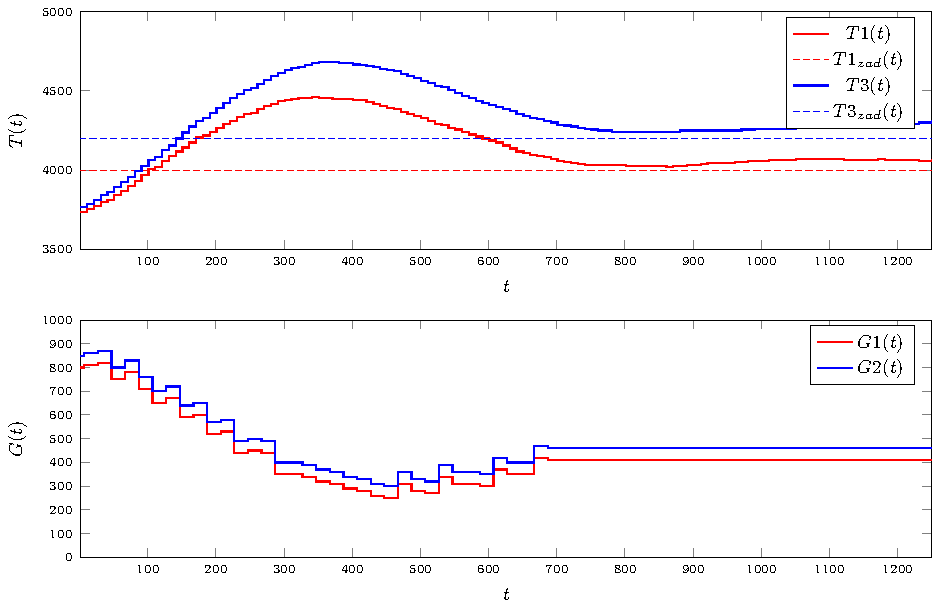
\includegraphics[scale=1]{../wykresy/zad3_pid.pdf}
	\caption{Regulator PID dla stanowiska grzejąco-chłodzącego}
	\label{zad3_pid}
\end{figure}

\chapter{Zad. 4}

Algorytm DMC w wersji oszczędnej obliczeniowo został zaimplementowany na sterowniku. Kod jest dostępny, tak jak w przypadku regulatora PID, w pliku programu gxworks3. Pobrane zostały dwie odpowiedzi skokowe, ponieważ odpowiedzi są symetryczne. Pobrane zostały odpowiedzi skokowe torów $T1(G1)$ oraz $T3(G1)$. Odpowiedź skokowa $T3(G2)$ jest identyczna jak odpowiedź skokowa $T1(G1)$, a odpowiedź skokowa $T1(G2)$ jest identyczna jak odpowiedź skokowa $T3(G1)$. Regulator DMC bardzo powoli dochodzi do wartości zadanej, jest to prawdopodobnie spowodowane zbyt dużą niedokładnością w reprezentacji liczb w sterowniku.

\begin{figure}[]
	\centering
	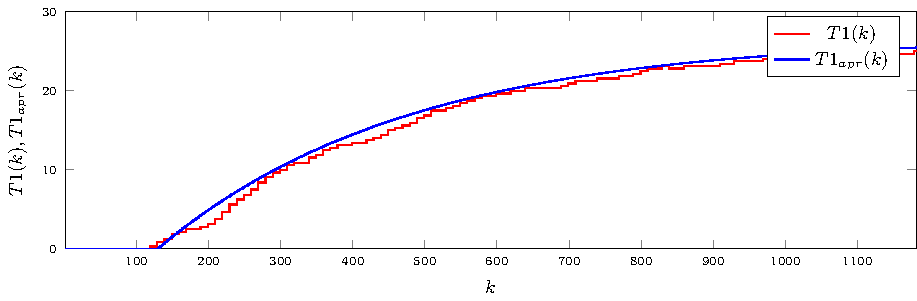
\includegraphics[scale=1]{../wykresy/zad4_odp1.pdf}
	\caption{Odpowiedź skokowa $T1(G1)$ i $T3(G2)$ dla $\Delta G = 20°C$}
	\label{zad4_odp1}
\end{figure}


\begin{figure}[]
	\centering
	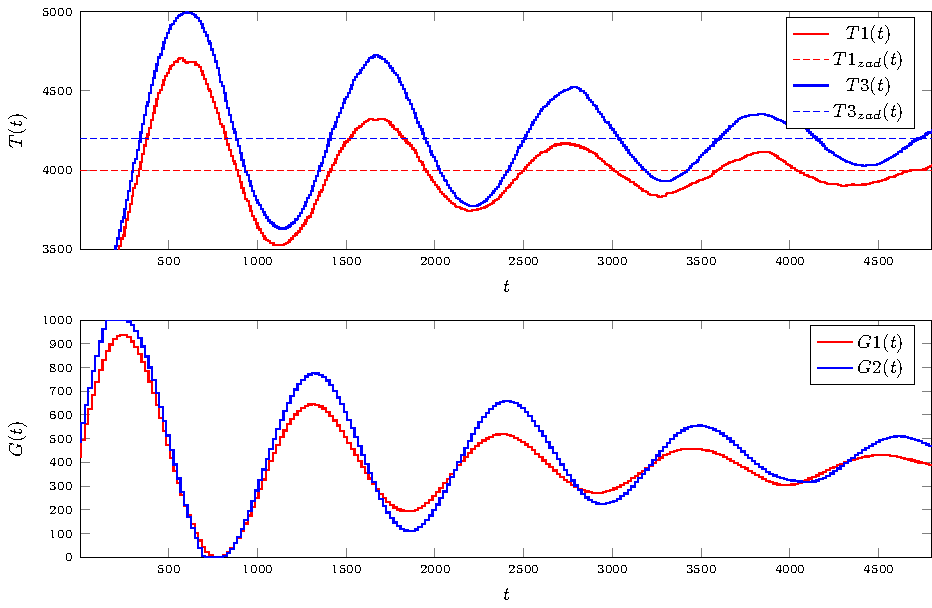
\includegraphics[scale=1]{../wykresy/zad4_dmc.pdf}
	\caption{Regulator DMC dla stanowiska grzejąco-chłodzącego}
	\label{zad4_pid}
\end{figure}


\chapter{Zad. 5}

Na panelu operatora zostały wyświetlone wartości mierzone, zadane oraz sterowanie. Dodatkowo, na panelu została wyświetlona grafika prezentująca obiekt. Wszystkie wartości są aktualizowane podczas pracy obiektu. Wyświetlone zostały też wartości parametrów dla regulatora PID. Sygnały mierzone oraz sterowanie są prezentowane w dwóch postaciach: jako wartość liczbowa oraz jako wypełnienie prostokąta kolorem.

\begin{figure}[]
	\centering
	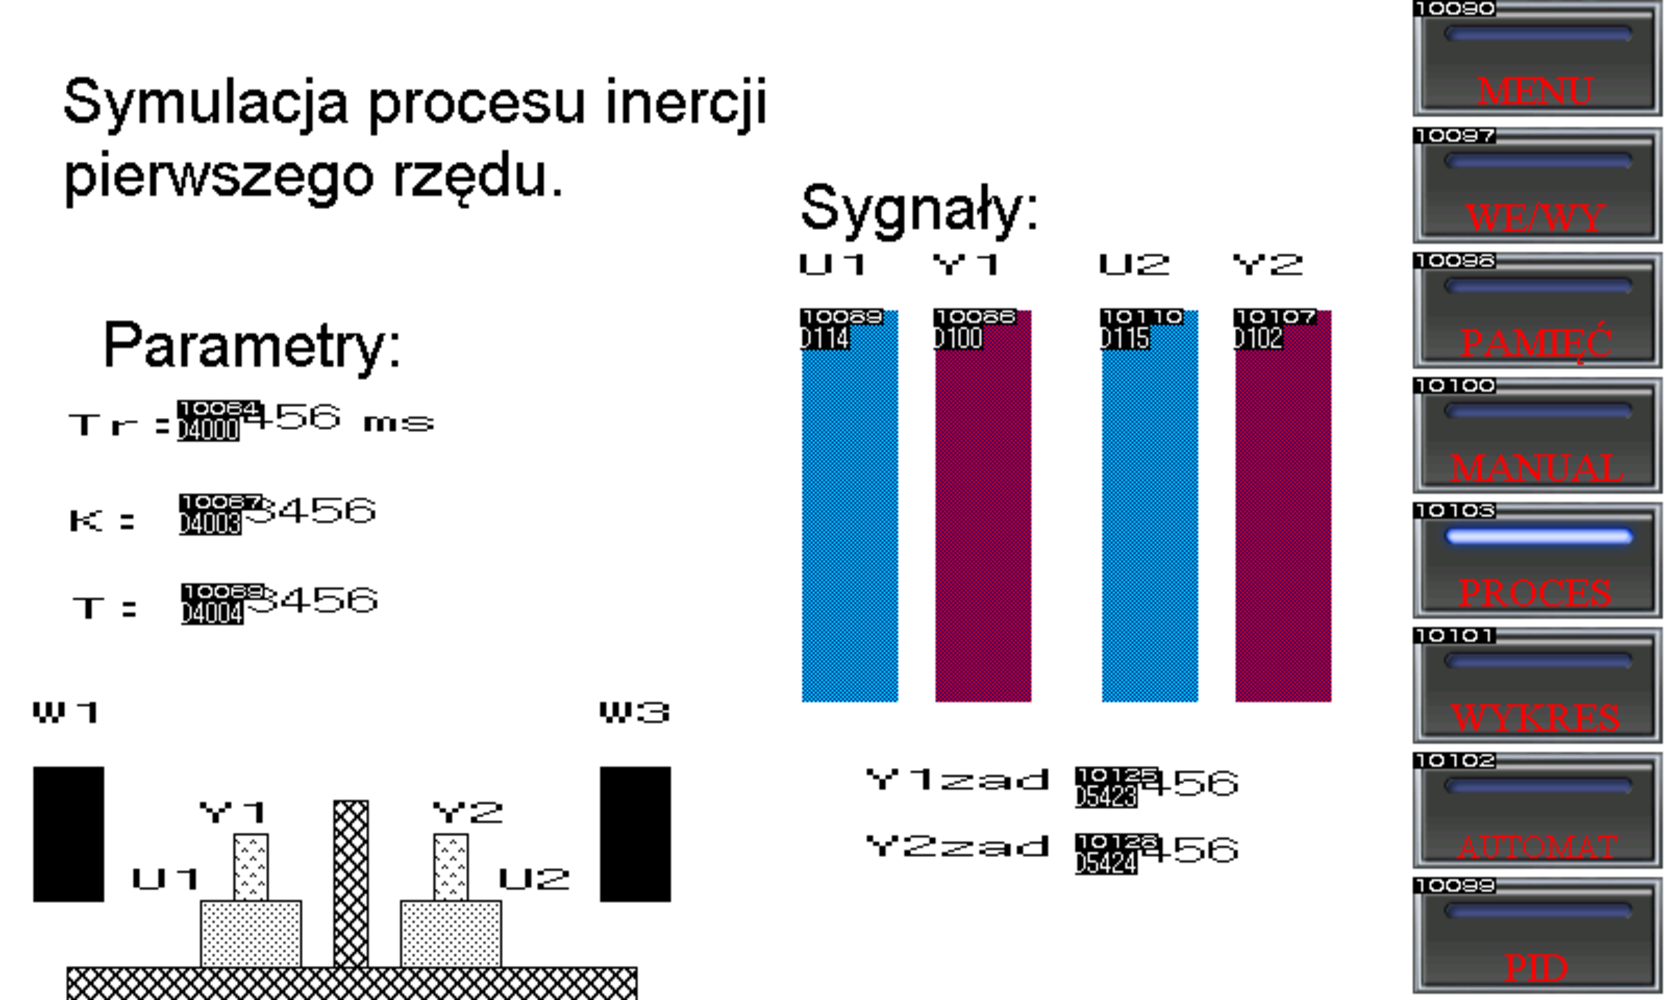
\includegraphics[scale=0.6]{../graphics2.pdf}
	\caption{Grafika na panelu sterownika dla stanowiska grzejąco-chłodzącego}
	\label{zad5_graph}
\end{figure}


\chapter{Zad. 6}

Został przygotowany automat stanów, na podstawie którego modyfikowane miały być wartości zadane. Sam automat został zaimplementowany w języku ST na sterowniku. Naciskanie odpowiednich przycisków powodowało przechodzenie pomiędzy poszczególnymi stanami automatu. Nie został on połączony z wartością zadaną procesu.

\begin{figure}[]
	\centering
	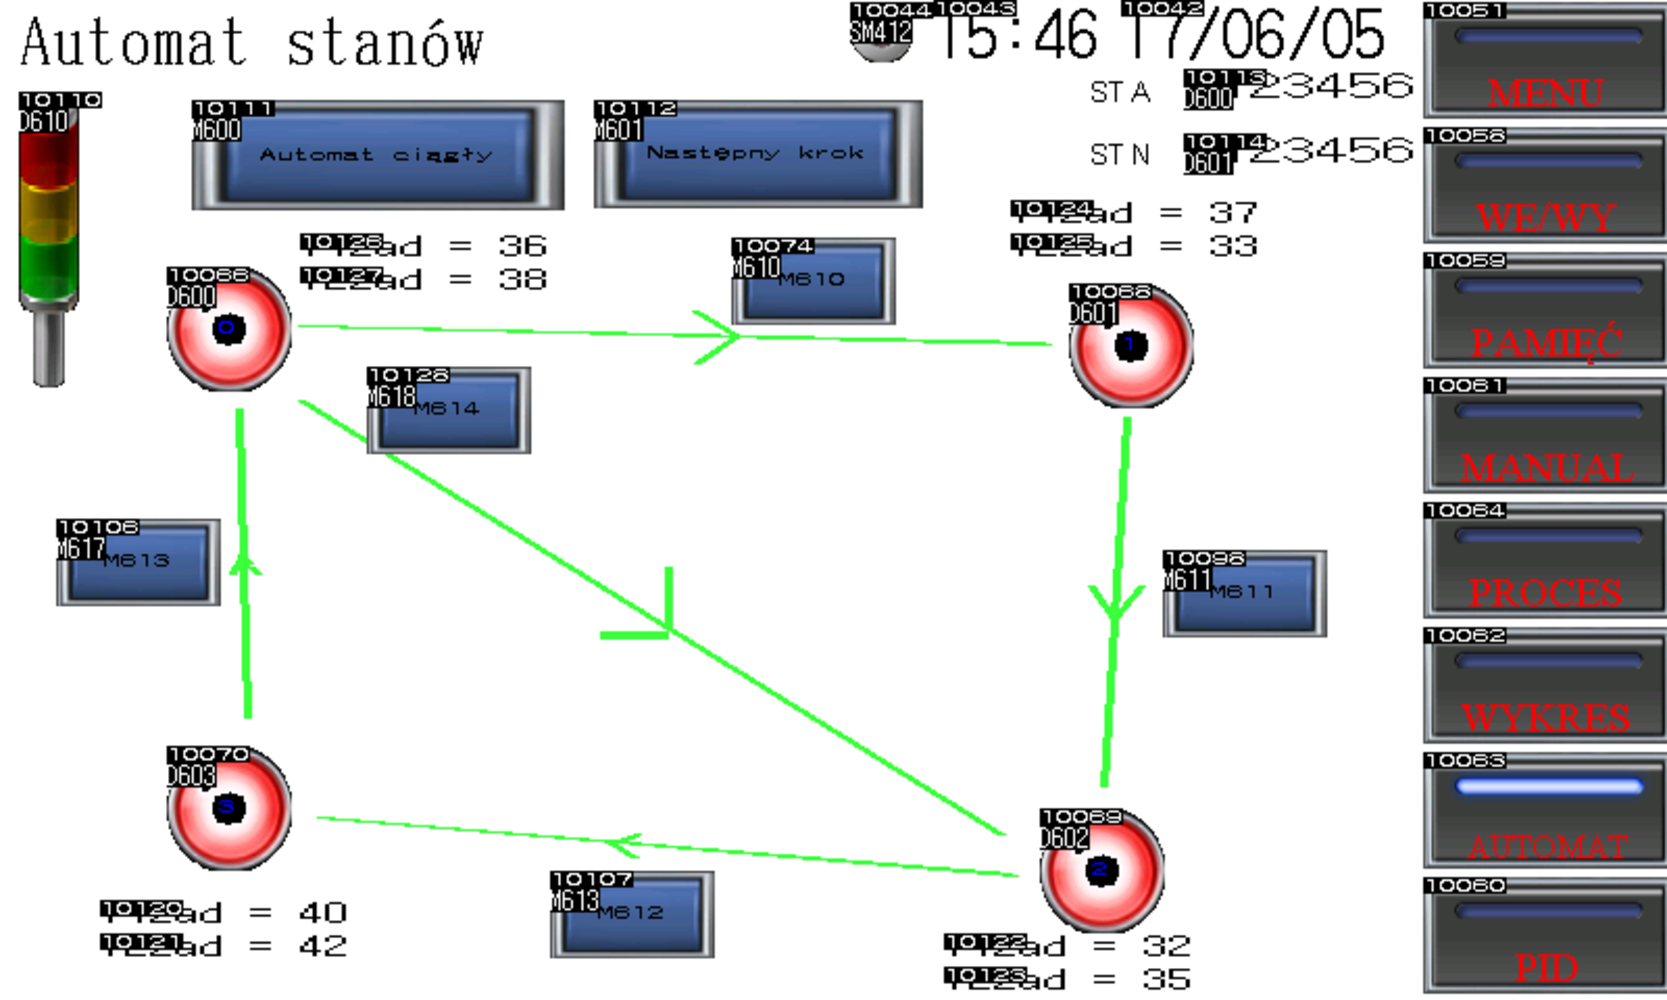
\includegraphics[scale=0.6]{../graphics.pdf}
	\caption{Automat stanów dla stanowiska grzejąco-chłodzącego}
	\label{zad6_graph}
\end{figure}


\chapter{Zad. 7}

Sterownik został skonfigurowany. Pracowaliśmy na stanowisku "TRAS" (śmigła). Wejście analogowe zostało odpowiednio skonfigurowane (dwukanałowy szybki licznik enkodera dla osi poziomej). Zostało również skonfigurowane wyjście PWM. Dla wyjścia PWM zakres został wybrany zgodnie z instrukcją: K200. Proces, który regulowaliśmy to wychylenie pionowe śmigieł.

\begingroup
\renewcommand{\cleardoublepage}{}
\renewcommand{\clearpage}{}

\chapter{Zad. 8}

Mechanizm zabezpieczający przed uszkodzeniem stanowiska został zaimplementowany jako ograniczenie na maksymalną wartość wypełnienia PWM. Nie zostały zaimplementowane ograniczenia na temperaturę stanowiska.


\chapter{Zad. 9}

Została wyznaczona charakterystyka statyczna. Na osi odciętych znajduje się wypełnienie PWM w sterowniku. Jest to część wypełnienia dla $5 kHz$, z negatywnym efektem. Wypełnienie PWM sygnału do stanowiska Inteco jest odwrotnie proporcjonalne do wypełnienia w sterowniku. Zakres PWM w sterowniku to $1 - 200$, gdzie $1$ to wartość maksymalna (100\% wypełnienia), a $200$ to wartość minimalna (0\% wypełnienia). Na osi rzędnych są wartości wyjścia enodera znajdującego się na osi poziomej (wskazuje on wychylenie w pionie). Wartości te są odwrotnie proporcjonalnie do wysokości, na jakiej znajduje się śmigło pracujące w osi pionowej. Wartość $-941$ to maksymalne wychelenie do góry tego śmigła (znajduje się ono w górze dla maksymalnego wypełnienia sygnału PWM sterujacego tym śmigłem), a wartość $-137$ to wartość minimalnego wychylenia.\\
Charakterystyka wskazuje, że do wypełniania ok. $-100$ ($50\%$) śmigło znajduje się w pozycji maksymalnego wychylenia. Charakterystyka jest silnie nieliniowa, ale ma w przybliżeniu liniowe przedziały: $<1,100)$ i $<100,200>$.


\begin{figure}[]
	\centering
	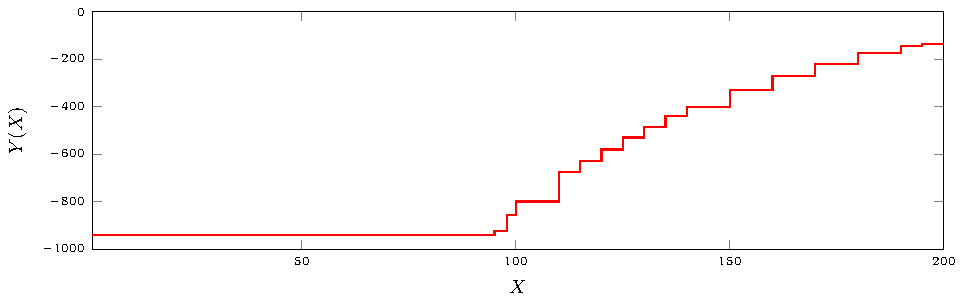
\includegraphics[scale=1]{../wykresy/zad9_chst.pdf}
	\caption{Charakterystyka statyczna stanowiska Inteco "TRAS"}
	\label{zad9_chst}
\end{figure}


\endgroup

\chapter{Zad. 10}

Regulator PID został dostosowany do pracy ze stanowiskiem Inteco. Jedyne zmiany, które były wymagane, to dostosowanie okresu próbkowania i zakresów. Dostrojenie regulatora było bardzo trudne z powodu nieliniowości procesu. Przyjęliśmy następującą strategię: założyliśmy punkt pracy jako poziomą pozycje śmigieł (wartość enkodera $-300$) i dostosowywaliśmy parametry regulatora (metodą inżynierską) do pracy w położeniu bliskim punktu pracy (do ok. 30° wychylenia). Po początkowym dostrojeniu blisko punktu pracy rozpoczęliśmy strojenie regulatora w pełnym zakresie. Parametry regulatora PID po około $30$ eksperymentach to: $K = 1$, $Ti = 50$, $Td = 1$. Przy regulacji PID zastosowaliśmy zerowanie enkodera w pozycji poziomej oraz odwrócenie znaku. Wykres sterowania został niestety nadpisany innymi danymi. Okres sterowania to $1 sekunda$. Regulator pomimo bardzo długiego okresu sterowania reguluje efektywnie. 

\begin{figure}[]
	\centering
	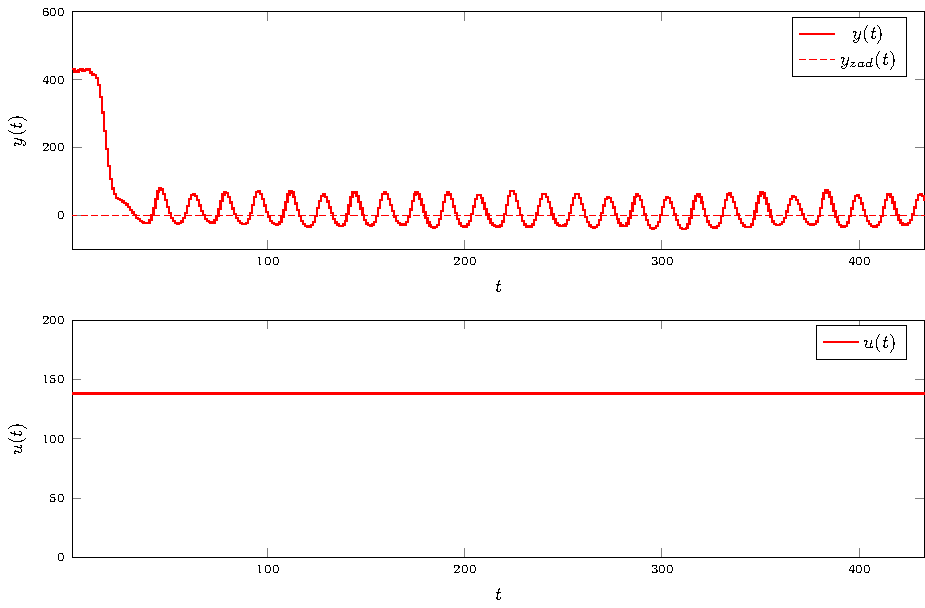
\includegraphics[scale=1]{../wykresy/zad10_pid.pdf}
	\caption{Regulator PID dla stanowiska Inteco}
	\label{zad10_pid}
\end{figure}

\chapter{Zad. 11}

Działanie wbudowanego regulatora PID okazało się lepsze, niż implementowanego przez nas. Te same nastawy regulatora w połączeniu z dużo krótszym okresem sterowania ($100 milisekund$) dały nam bardzo dobry regulator. Parametry zastosowane w funkcji PID to wypełnienie sygnału PWM (MV), wartość zadana (SV) oraz pomiar z enkodera(PV). Nie został sprawdzony wpływ ograniczeń na działanie obu wersji regulatora. Prawdopodobnie zmniejszenie maksymalnego wypełnienia PWM do wartości ok. 55\% wprowadziłoby poprawę pracy regulatora z powodu niwelacji nieliniowości obiektu.

\begin{figure}[]
	\centering
	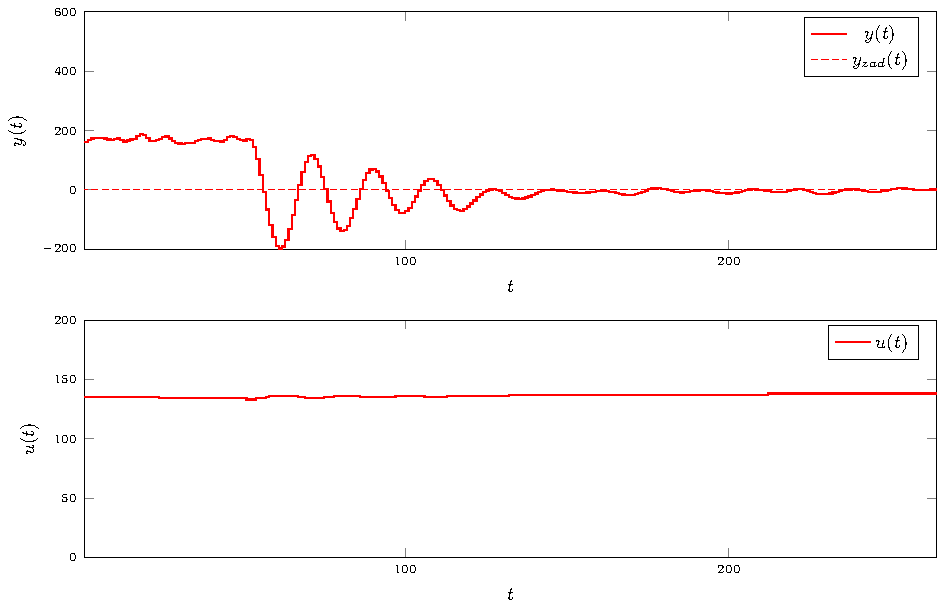
\includegraphics[scale=1]{../wykresy/zad11_pid.pdf}
	\caption{Wbudowany regulator PID dla stanowiska Inteco}
	\label{zad11_pid}
\end{figure}



\chapter{Zad. 12 i 13}

Dostosowano graf przejść automatu stanów oraz wizualizację procesu. Automat stanów nie został połączony z wartością zadaną.

Na panelu operatora zostały wyświetlone wartość mierzona (enkoder), zadana oraz sterowanie (wartość PWM w sterowniku). Tak jak w przypadku obiektu grzejąco-chłodzącego, została stworzona grafika prezentująca proces.

\begin{figure}[]
	\centering
	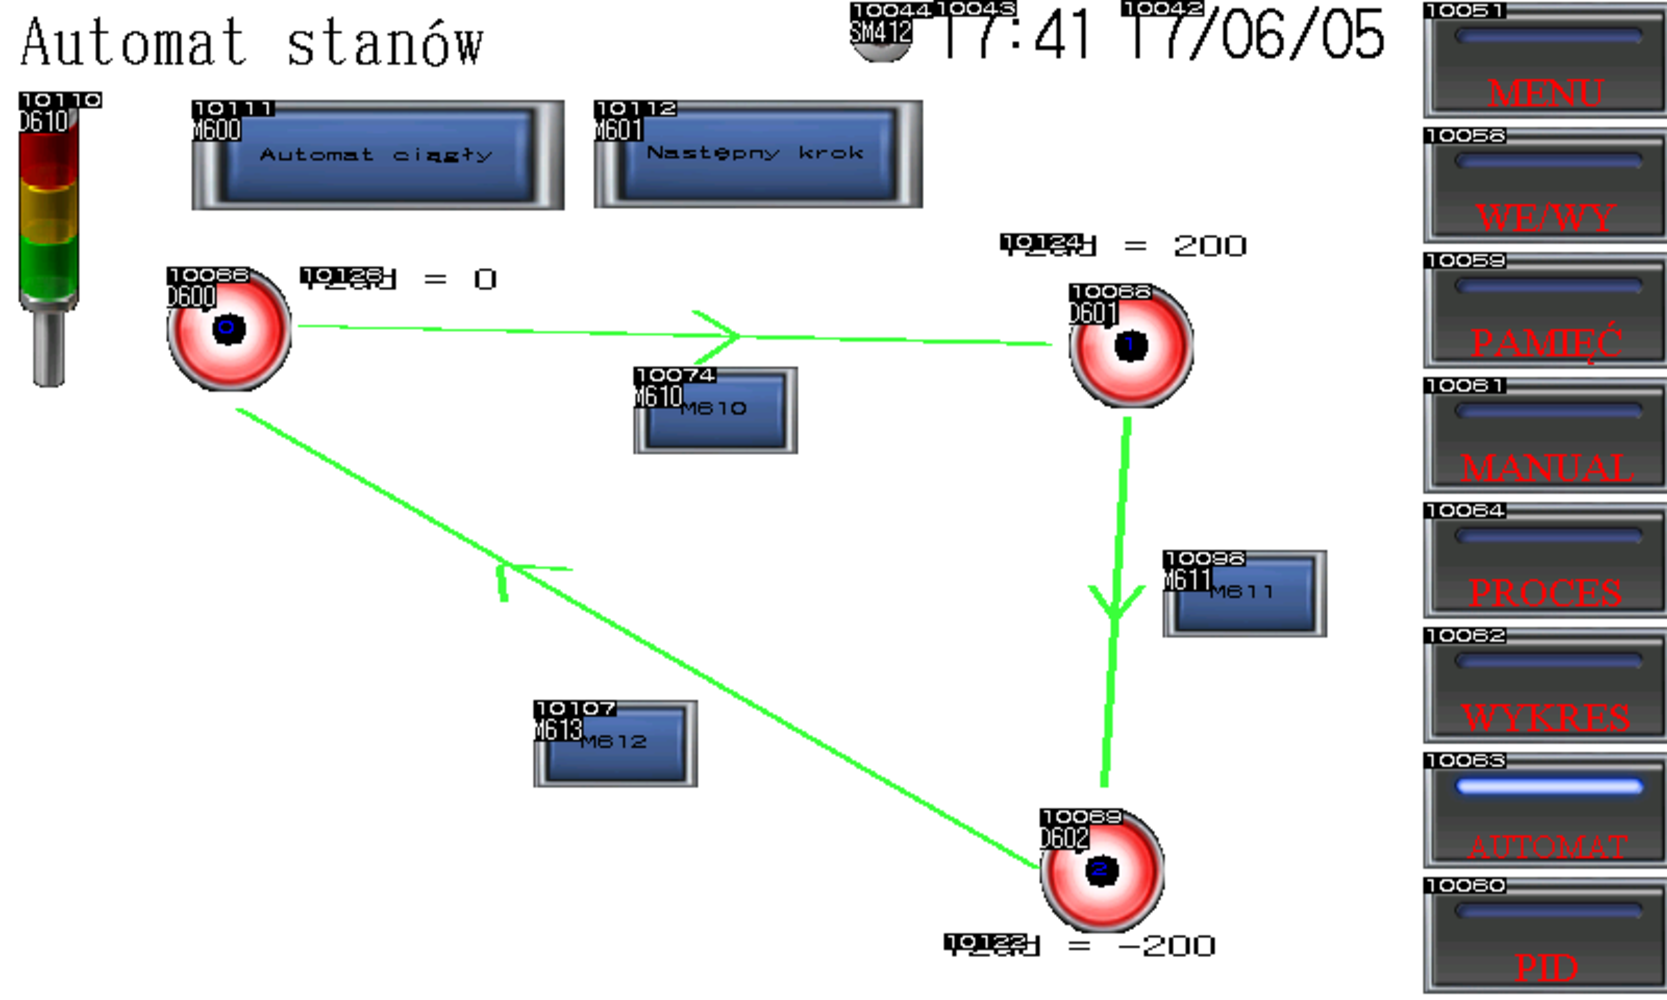
\includegraphics[scale=0.6]{../intecographics.pdf}
	\caption{Automat stanów dla stanowiska grzejąco-chłodzącego}
	\label{zad12_graph}
\end{figure}


\begin{figure}[]
	\centering
	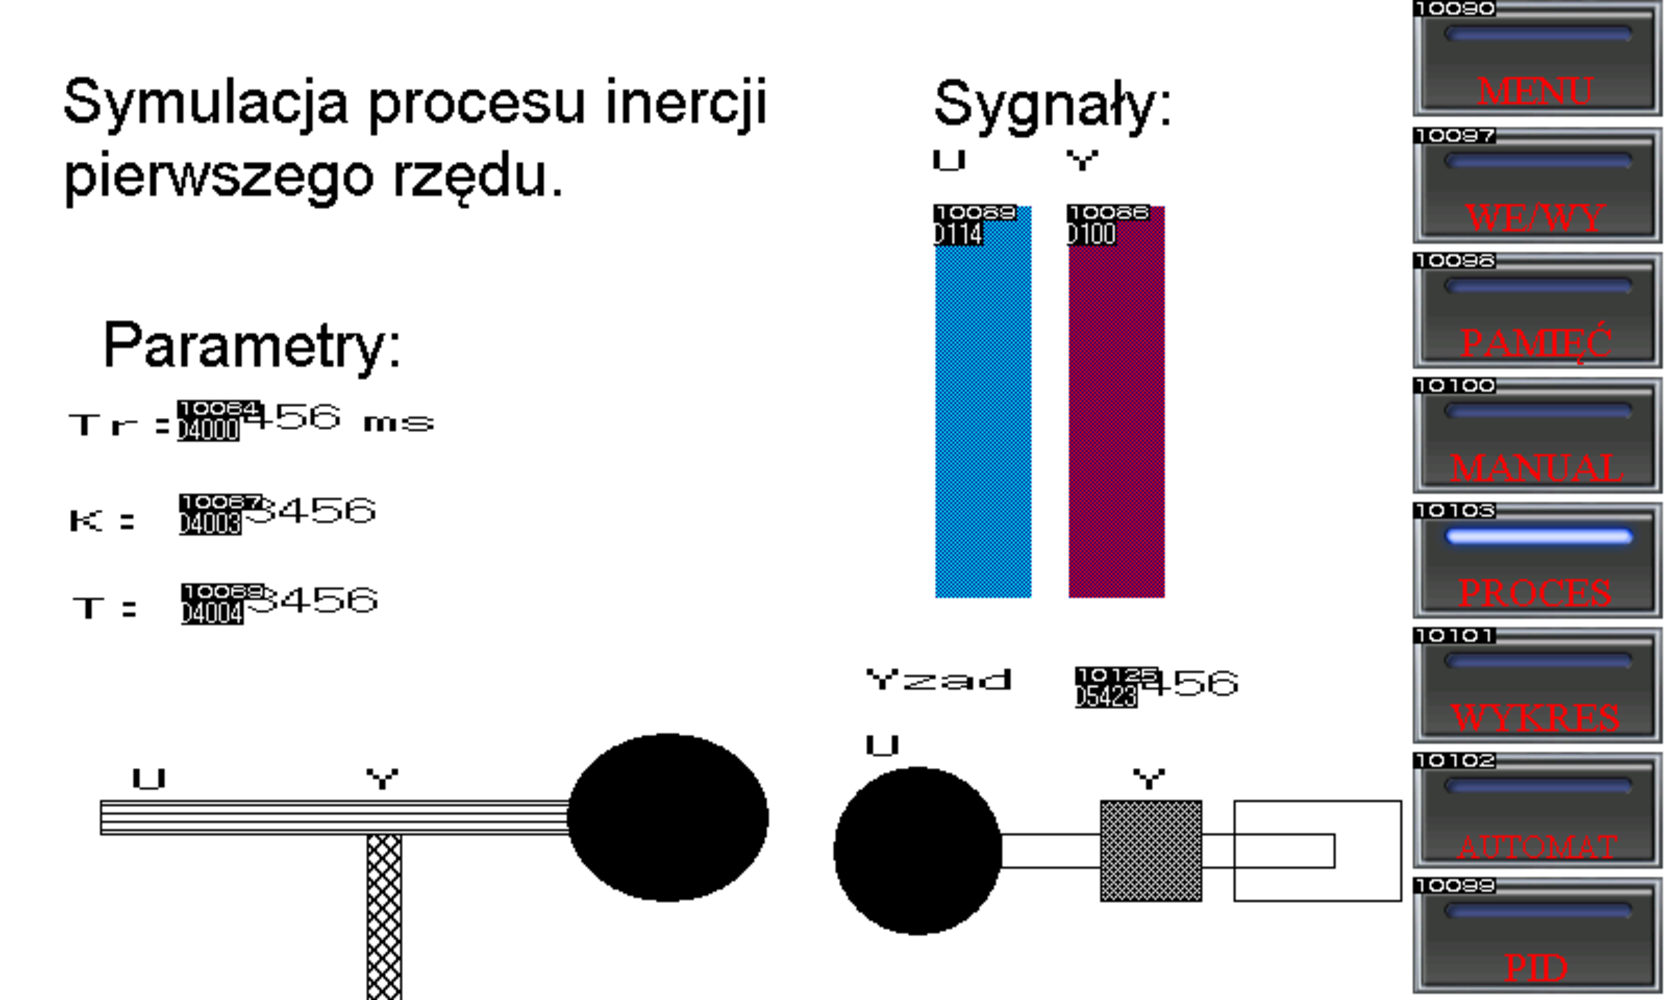
\includegraphics[scale=0.6]{../intecographics2.pdf}
	\caption{Grafika na panelu sterownika dla stanowiska Inteco}
	\label{zad13_graph}
\end{figure}

%\endgroup
\end{document}
